\chapter{First and Second Derivatives and the Shape of a Function}
\section{Using first derivatives to describe a function}
\subsection{Critical Values}

Let's re-examine our graph showing the height of a hammer tossed in the air:


\begin{figure}
\centering
\begin{tikzpicture}
    \begin{axis}[ymin=0,ymax=1.4, xmin=0, xmax=1.2, axis lines=left]
    \addplot[blue, samples=50, domain=0:1.2]{5*x-4.9*x^2};
    \end{axis}
\end{tikzpicture}
\caption{Height of a hammer over time}
\label{ref:hammerh}
\end{figure}


As you can see, the hammer reaches its peak around $t \approx 0.5s$ (see 
figure \ref{ref:hammerh}). Let's add tangent lines just before and after the 
peak of the hammer's path, so we can more easily examine how the slope of the 
graph changes:

\begin{figure}
\centering
\begin{tikzpicture}
    \begin{axis}[ymin=0,ymax=1.4, xmin=0, xmax=1.2, axis lines=left]
    \addplot[blue, samples=50, domain=0:1.2]{5*x-4.9*x^2};
    \addplot[red, samples=50, domain=0.31:0.49]{1.08*x-0.4*1.08+1.216};
    \addplot[red, samples=50, domain=0.11:0.29]{3.04*x-0.2*3.04+0.804};
    \addplot[red, samples=50, domain=0.61:0.79]{-1.86*x+1.86*0.7+1.099};
    \addplot[red, samples=50, domain=0.81:0.99]{-3.82*x+0.9*3.82+0.531};
    \end{axis}
\end{tikzpicture}
\caption{height of a hammer over time}
\label{ref:hammerh2}
\end{figure}


In figure \ref{ref:hammerh2}, we see that the slope changes from positive to 
negative as $t$ increases. That implies that $f'(t)$ also changes from positive 
to negative. In fact, at the highest point of the hammer's flight, the slope 
(and therefore $f'(t)$) is exactly zero! In general, 
\begin{enumerate}
	\item If $f'(x)>0$ on an interval, then $f(x)$ is increasing on that 
	interval.
	\item If $f'(x)<0$ on an interval, then $f(x)$ is decreasing on that 
	interval. 
\end{enumerate}

Example 1: Find where the function $f(x) = 3x^4-4x^3-12x^2+5$ is increasing. 

Solution: We want to find the intervals where $f'(x)>0$. First, we take the 
derivative to find $f'(x)$:
$$f'(x) = 12x^3-12x^2-24x$$

It will be easier to analyze the value of $f'(x)$ if we factor it so:
$$f'(x) = 12x(x-2)(x+1)$$

To determine where $f'(x)>0$, we start by finding where $f'(x)=0$ (in this 
case, this is true when $x=-1, 0, 2$). These values of $x$ are called \textit{
critical values}, and we will use them to divide $f'(x)$ into intervals. 
(Critical values are also called critical numbers, and we will use both in 
this text.) On each of these intervals, $f'(x)$ must be always positive or 
always negative. This is shown in the graph below:

\begin{figure}
	\begin{tikzpicture}
		\begin{axis}[xmin=-2, xmax=3, axis lines=center]
		\addplot[blue, samples=100, domain=-2:3]{12*x*(x-2)*(x+1)};
		\addplot[red, dashed, samples=50]coordinates {(-1, -75) (-1, 125)};
		\addplot[red, dashed, samples=50]coordinates {(0, -75) (0, 125)};
		\addplot[red, dashed, samples=50]coordinates {(2, -75) (2, 125)};
		\end{axis}
	\end{tikzpicture}
	\caption{$f'(x)$ with critical values}
	\label{fig:critval1}
\end{figure}


As you can see in figure \ref{fig:critval1}, $f'(x)>0$ on two intervals: $x 
\in (-1, 0) $ and $x \in (2, \infty)$. These are open intervals because $f'(x) 
= 0$ at $x = -1$, $x = 0$, and $x = 2$. But what if we had a more complex 
function, or didn't have the resources to graph it? We can use a table to help 
us analyze the value of $f'(x)$ (and therefore the behavior of $f(x)$). For 
each interval around the critical values, we can determine if $f'(x)$ is 
positive or negative by noting the value of the factors of $f'(x)$, which are 
$12x$, $x-2$, and $x+1$ in this case. For example, for $x < -1$, $12x < 0$, $(
x - 2) < 0$, and $(x + 1) < 0$. Three negatives multiplied together is also 
negative. Therefore, for $x<-1$, $f'(x)$ is negative and $f(x)$ is decreasing. 
We can analyze all of the intervals similarly and log the results in a table:

\begin{tabular}{c | c | c |c|c|c}
\hline
$x$ & $12x$ & $x-2$ & $x+1$ & $f'(x)$ & $f(x)$ \\
$x<-1$ & negative & negative & negative & negative &decreasing\\
$-1<x<0$ & negative & negative & positive & positive & increasing \\
$0<x<2$ & positive & negative & positive & negative & decreasing \\
$2<x$ & positive & positive & positive & positive & increasing\\
\end{tabular}

Notice the table method yields the same result as examining the graph: $f(x)$ 
is increasing for $x\in (0, -1)$ and $x \in (2, \infty)$, which can also be 
written as $x \in (-1, 0) \cup (2, \infty)$. 

\begin{Exercise}[label=critval1]
	Let $g$ be the function given by $g(x) = x^2e^{kx}$, where $k$ is a constant. 
	For what value(s) of $k$ does $g$ have a critical value at $x=\frac{2}{3}$?
\end{Exercise}

\begin{Answer}[ref=critval1]
	Recall that critical values are values of $x$ where $g'(x) =0$ or is 
	undefined. We need to find an expression for $g'(x)$, set it equal to zero 
	when $x=\frac{2}{3}$, and solve for $k$. 
	$$g'(x) = x^(2)[k*\exp{kx}]+\exp{kx}[2x]$$
	$$g'(\frac{2}{3})=(\frac{2}{3})^2[k*\exp{\frac{2k}{3}}]+\frac{4}{3}\exp{\frac{
	2k}{3}}=0$$
	$$\frac{4k}{9}e^{\frac{2k}{3}}+\frac{4}{3}e^{\frac{2k}{3}}=0$$
	$$(\frac{4k}{9}+\frac{4}{3})e^{\frac{2k}{3}}=0$$
	There are no real values of $k$ such that $e^{\frac{2k}{3}}=0$, therefore, we 
	will examine the other factor:
	$$\frac{4k}{9}+\frac{4}{3}=0$$
	$$\frac{4k}{9}=\frac{-4}{3}$$
	$$\frac{k}{3}=-1$$
	$$k=-3$$
	Therefore, $g(x)$ has a critical value at $x=\frac{2}{3}$ when $k=-3$.
\end{Answer}

\subsection{Local Extrema}
Examine the graphs of $x^2$, $\sin{x}$, and $y=\sqrt{4-x^2}$ below. Each has a 
dot at a local extreme (either a local minimum or local maximum). Sketch what 
you think the tangent line to the graph would be at each local extreme. Use 
this to estimate the value of the derivative at that point. 

%FIXME format graphs side-by-side horizontally
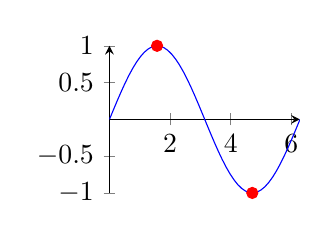
\begin{tikzpicture}
	\begin{axis}[width=4cm, xmin=0, xmax=6.28, axis lines=center]
	\addplot[blue, samples=50, domain=0:6.28]{sin(deg(x))};
	\addplot[red, mark=*]coordinates {(1.57, 1)};
	\addplot[red, mark=*]coordinates{(4.71, -1)};
	\end{axis}
\end{tikzpicture}

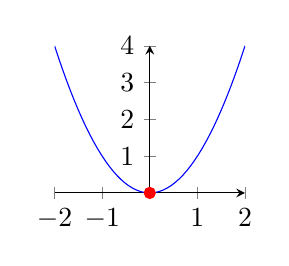
\begin{tikzpicture}
	\begin{axis}[width=4cm, xmin=-2, xmax=2, axis lines=center]
	\addplot[blue, samples=50, domain=-2:2]{x^2};
	\addplot[red, mark=*]coordinates{(0, 0)};
	\end{axis}
\end{tikzpicture}

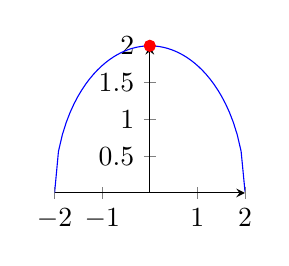
\begin{tikzpicture}
	\begin{axis}[width=4cm, xmin=-2, xmax=2, axis lines=center]
	\addplot[blue, samples=50, domain=-2:2]{sqrt(4-x^2)};
	\addplot[red, mark=*]coordinates{(0, 2)};
	\end{axis}
\end{tikzpicture}

You should notice that all of the tangent lines are horizontal. Since the 
tangent lines at these local extrema have a slope of $0$, that tells us $f'(x) 
= 0$ at these points as well. In fact, for \textit{all} local minima and maxima, 
the value of the derivative is zero at that point. However, the converse 
statement is not necessarily true; just because the derivative is zero at 
some $x = c$, it does not mean there is a local extrema at $f(c)$. Consider 
$f(x) = x^3+3$, shown in figure  \ref{fig:nonextrema}:

\begin{figure}
	\centering
	\begin{tikzpicture}
		\begin{axis}[axis lines=center]
		\addplot[blue, samples=50, domain=-1:1]{x^3+3};
		\addplot[red, mark=*]coordinates{(0, 3)};
		\addplot[red, samples=50]coordinates{(-0.25, 3) (0.25,3)};
		\end{axis}
	\end{tikzpicture}
	\caption{$f(x) = x^3+3$}
	\label{fig:nonextrema}
\end{figure}


At $x=0$, $f'(x)=0$, but there is not a local extreme. For a local extreme to 
exist, the graph of $f(x)$ must change from increasing to decreasing, or vice 
versa. Look closely at figure \ref{fig:nonextrema}: the function is increasing 
for $x<0$ and $x>0$. Another way of saying this is to note that the graph of 
$f'(x)$ touches but does not cross the x-axis in this case:

\begin{figure}
	\centering
	\begin{tikzpicture}
		\begin{axis}[axis lines = left]
		\addplot[blue, samples=50, domain=-2:2]{3*x^2};
		\end{axis}
	\end{tikzpicture}
	\caption{$f'(x) = 3x^2$}
	\label{fig:touch}
\end{figure}


If $f(x)$ changes from increasing to decreasing, then $f'(x)$ is changing from 
positive to negative (i.e. crossing the x-axis). Look at the derivative of 
$f(x) = \sin{x}$, $f'(x)=\cos{x}$, presented in figure \ref{fig:fprimecos}. 
The x-values where local extrema exist on $f(x)$ are marked in red (recall 
$\sin{x} = \pm 1$ when $x=\frac{n\pi}{2}$):

\begin{figure}
	\centering
	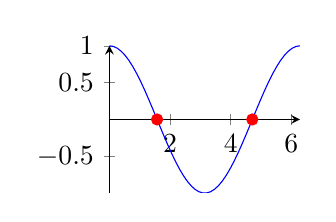
\begin{tikzpicture}
		\begin{axis}[width=4cm, xmin=0, xmax=6.28, axis lines=center]
		\addplot[blue, samples=50, domain=0:6.28]{cos(deg(x))};
		\addplot[red, mark=*]coordinates {(1.57, 0)};
		\addplot[red, mark=*]coordinates{(4.71, 0)};
		\end{axis}
	\end{tikzpicture}
	\caption{$f'(x) = \cos{x}$}
	\label{fig:fprimecos}
\end{figure}


As you can see, local extrema are indicated when $f'(x)$ crosses the x-axis. 
If $f'(x)$ is negative to the left of $x=c$ and positive to the right, then 
$f(x)$ has a local minimum at $x=c$. On the other hand, if $f'(x)$ is positive 
to the left of $x=c$ and negative to the right, then $f(x)$ has a local 
maximum at $x=c$. Any value of $x=c$ where $f'(c) = 0$ is called a \textbf{
critical number} or a \textbf{critical value}. Values where $f(c)$ does not 
exist are also a critical numbers. 

\subsection{Practice: Interval of Increasing and Decreasing, Local Extrema}
\begin{Exercise}
    [label=incdec1]
    Let $f$ be the function given by $f(x) = 300x-x^3$. On which of the 
    following intervals is $f$ increasing?
\end{Exercise}

\begin{Answer}
    [ref=incdec1]
    First, we will find $f'$ and set it equal to zero: $$f'(x) = 300 - 3x^2 = 
    0$$ $$300=3x^2 \rightarrow x=\pm \sqrt{100} = \pm10$$ (Note: $f'(x) = 3(10 
    - x)(10 + x)$, which implies roots at $x=\pm10$. Now, we will evaluate the 
    value of $f'(x)$ for $x < -10$, $-10 < x < 10$, and $ x >10$. 
    \begin{center}
        \begin{tabular}{c|c|c|c|c}
        Value of $x$ & (10-x) & (10+x) & $f'(x)$ & $f(x)$ behavior\\
         $x<-10$    &  positive & negative& negative & decreasing\\
         $-10<x<10$    & positive & positive& positive& increasing\\
         $x>10$ & negative & positive & negative & decreasing
        \end{tabular}
    \end{center}
    Therefore, the function is increasing on the interval $x \in [-10, 10]$ 
    because $f'(x) >0$ for $x \in [-10, 10]$.
\end{Answer}

\begin{Exercise}[label=locext1]
Find the intervals on which $f(x)=x^3-3x^2-9x+4$ is increasing or decreasing. 
Then, find all local minimum and/or maximum values of $f(x)$. 
\end{Exercise}

\begin{Answer}[ref=locext1]
Given $f(x)=x^3-3x^2-9x+4$, it follows that $f'(x)=3x^2-6x-9$. Factoring, we 
find that $f'(x) = 9(x-3)(x+1)$ and $f'(x) = 0$ when $x=3$ and $x=-1$. We 
construct our table to help us analyze the value of $f'(x)$ and behavior of 
$f(x)$ on the whole domain of the function:
\begin{center}
	\begin{tabular}{c|c|c|c|c}
		Value of $x$ & $(x-3)$ & $(x+1)$ & $f'(x)$ & $f(x)$ behavior\\
		$x<-1$ & negative & negative & positive & increasing\\
		$-1<x<3$ & negative & positive & negative & decreasing\\
		$x>3$ & positive & positive & positive & increasing
	\end{tabular}
\end{center}
So, $f(x)$ is increasing for $x \in (-\infty, -1) \cup (3, \infty)$ and 
decreasing for $x \in (-1, 3)$. Since $f'(-1)=0$ and changes from positive to 
negative, $f(x)$ has a local maximum at $x=-1$. And since $f'(3)=0$ and 
changes from negative to positive, $f(x)$ has a local minimum at $x=3$.
\end{Answer}



\subsection{Global Extrema}
Now that we've learned how to identify local minima and maxima, let's expand 
the discussion to include global extrema. A global extreme is an absolute 
minimum or maximum value of a function over a particular interval or the entire 
domain of the function. Let's examine the graph of $f(x) = x^4-5x^3+6x^2$ over 
the domain $x \in [-1,4]$.

\begin{figure}[htbp]
  \centering
  \begin{tikzpicture}
    \begin{axis}[clip=false,
	  xmin=-1, xmax=4,
      axis lines = middle,
      xlabel = \(x\),
      ylabel = \(f(x)\),
      samples = 100,
    ]
    \addplot [blue, smooth, domain=-1:4] {x^4-5*x^3+6*x^2}
    node[color=black, left, pos=0.0]{$(-1, 12)$}
    node[color=black, left, pos=0.95]{$(4, 32)$};
    %fixme label local minima and maximum
    \addplot[red, mark=*]coordinates{(-1,12)};
    \addplot[red, mark=*]coordinates{(0,0)};
    \addplot[red, mark=*]coordinates{(1.157,2.08)};
    \addplot[red, mark=*]coordinates{(2.593,-1.623)};
    \addplot[red, mark=*]coordinates{(4,32)};
    \end{axis}
  \end{tikzpicture}
  \caption{Graph of \( f(x) = x^4-5x^3+6x^2 \) }
  \label{fig:globalext}
\end{figure}

As you can see in figure \ref{fig:globalext}, $f(x)$ has two local minima and 
one local maximum. Additionally, the endpoints are labeled. To determine the 
\textit{global} extrema, we need to examine the any local extrema (identified 
here graphically, but you can also identify them mathematically using that you 
learned in the "Local Extrema" subsection) \textbf{and} the endpoints of the domain (or 
the function's behavior at $\pm \infty$, if you are Notet restricted to a specific 
domain). 

In the case of $f(x) = x^4-5x^3+6x^2,\text{ }for x\in [-1,4]$, the global 
maximum value is 32 at $x=4$ and the global minimum is -1.623 at $x=2.593$. 

If a function is continuous on an interval, then there must exist a global 
maximum and global minimum on that interval. These global extrema may also be 
local extrema (as is the case for $f(2.593)$ in the example above) or not (as 
is the case for $f(4)$). Applying the Closed Interval Method is a 
straightforward way to identify global (absolute) extrema. To find the global 
extrema of a continuous function, $f$, on a closed interval $[a, b]$:
\begin{enumerate}
	\item Find the values of $f$ at the critical numbers of $f$ in $(a, b)$.
	\item Find the values of $f$ at the endpoints of the interval.
	\item The largest of the values from steps 1 and 2 is the absolute maximum; 
	the smallest of the values is the absolute minimum.
\end{enumerate}

Let's use the Closed Interval Method to determine the global extrema for the 
function $g(x) = x-3\sin{x}$ on the interval $x \in [0, 2\pi]$.

To find the value of $g$ at any critical numbers, we must first identify the 
critical numbers. Recall that critical numbers are values where the first 
derivative of the function is $0$ or does not exist. To find critical numbers, 
we set $g'$ equal to $0$:
$$g'(x) = 1-3\cos{x}=0$$
$$3\cos{x} = 1$$
$$\cos{x} = \frac{1}{3}$$
$$x=1.23, 5.052$$
Now, we substitute these critical numbers back into $g(x)$:
$$g(1.23) \approx -1.60$$
$$g(5.052) = 7.881$$

Now we need to check the endpoints:
$$g(0) = 0-3*0 = 0$$
$$g(2\pi) = 2\pi - 3*0 = 2\pi \approx 6.28$$

The results are presented in the table below:

\begin{tabular}{c | c}
$x$ & $g(x)$\\
0 & 0\\
1.23 & -1.60\\
5.052 & 7.881\\
6.28 & 6.28\\
\end{tabular}

Therefore, for $g(x) = x-3\sin{x}$ on the interval $x \in [0, 2\pi]$, the 
global maximum is $g(5.052) = 7.881$ and the global minimum is $g(1.23) = 
-1.60$. 

\subsection{Practice: Global Extrema}
\begin{Exercise}[label=gloext1]
Let $f$ be the function defined by $f(x) = \frac{\ln{x}}{x}$. What is the 
absolute maximum value of $f$?
\end{Exercise}

\begin{Answer}[ref=gloext1]
First, we identify any critical numbers:
$$f'(x) = \frac{x*(\frac{1}{x})-\ln{x}*1}{x^2} = \frac{1-\ln{x}}{x^2}$$
Recall that critical numbers are values where $f'(x)=0$ or does not exist. 
We might identify $x=0$ as a critical number, but the presence of $\ln{x}$ 
limits the domain of the function to $x \in (0, \infty)$, excluding $x=0$. 
For all $x \in (0, \infty)$, $f'(x)$ exists. So, we look for values where 
$f'(x) = 0$.
$$\frac{1-\ln{x}}{x^2}=0$$
$$1-\ln{x}=0$$
$$1=\ln{x}$$
$$x=e$$

Finding the value of $f(x)$ at $x=e$: 
$$f(e) = \frac{\ln{e}}{e}=\frac{1}{e}$$
Because the domain of $f(x)$ is on an \textit{open interval}, instead of 
checking the endpoints directly, we'll take the limits as $x$ approaches $0$ 
and $\infty$.
$$\lim_{x\to 0}\frac{\ln{x}}{x}=-\infty<\frac{1}{e}$$
$$\lim_{x \to \infty}\frac{\ln{x}}{x}=0<\frac{1}{e}$$

Therefore, the absolute maximum values of $f(x) = \frac{\ln{x}}{x}$ is $\frac{
1}{e}$ at $x=e$. 
\end{Answer}

\begin{Exercise}[label=gloext2]
Find the global minimum and maximum values on the stated interval.
\begin{enumerate}
	\item $f(x) = 12+4x-x^2$, $[0,5]$
	\item $f(t) = \frac{\sqrt{t}}{1+t^2}$, $[0, 2]$
	\item $f(t) = 2\cos{t} + \sin{2t}$, $[0, \frac{\pi}{2}]$
	\item $f(x) = \ln{x^2+x+1}$, $[-1, 1]$
\end{enumerate}
\end{Exercise}

\begin{Answer}[ref=gloext2]
\begin{enumerate}
	\item $f'(x) = 4-2x$ and to find the critical numbers, we set $f'(x)=0$:
$$4-2x=0$$
$$x=2$$
We evaluate $f(x)$ at $x=0, 2, 5$:
$$f(0) = 12+4(0)-0^2=12$$
$$f(2) = 12+4(2)-2^2=12+8-4=16$$
$$f(5) = 12+4(5)-5^2=12+20-25=7$$
Therefore, the global maximum is $f(2) = 16$ and the global minimum is $f(5) = 7$.
\item %fixme complete answer key for gloext2
\end{enumerate}
\end{Answer}

\section{Sketching f from f'}
Now that we know how the shape of $f$ is related to the value of $f'$, we can 
predict the shape of $f$ if we are given $f'$. Take the example $f'(x) = -(x-1)
(x-5)$, shown in figure \ref{fig:sketchf1}:

\begin{figure}[htbp]
	\centering
	\begin{tikzpicture}
		\begin{axis}[axis lines= center, xmin=-0.5, xmax=6.5]
		\addplot[blue, samples=50, domain=0:6]{-(x-1)*(x-5)};
		\end{axis}
	\end{tikzpicture}
	\caption{Graph of $f'=-(x-1)(x-5)$}
	\label{fig:sketchf1}
\end{figure}

Using the graph of $f'$, we can construct an approximate sketch of $f$. First, 
let's identify the critical numbers. Where does $f'=0$? Take a second to 
examine the graph of $f'$ above and jot down what you think the critical 
numbers are.

You should recall that critical numbers are x-values where $f'=0$. Examining 
the graph of $f'$, we see that $f'=0$ at $x=1$ and $x=5$. We can now use a 
table to describe the behavior of $f$:

\begin{tabular}{c|c|c|c|c}
$x$ & $x-1$ & $x-5$ & $f'$ & behavior of $f$\\
$x<1$ & negative & negative & negative & decreasing\\
$x=1$ & zero & negative & zero & local minimum\\
$1<x<5$ & positive & negative & positive & increasing\\
$x=5$ & positive & zero & zero & local maximum\\
$x>5$ & positive & positive & negative & decreasing\\
\end{tabular}

We can use this information to sketch a possible graph of $f$. We start by 
noting the location of local extrema:
\begin{figure}[htbp]
	\centering
	\begin{tikzpicture}
		\begin{axis}[xmin=-0.5, xmax=7, axis lines = center]
		\addplot[red, dashed, samples=50]coordinates{(1,-4) (1, 4)};
		\addplot[red, dashed, samples=50]coordinates{(5, -4) (5, 4)};
		\end{axis}
	\end{tikzpicture}
	\caption{Possible graph of $f$}
	\label{fig:sketchf2}
\end{figure}

We know there is a local minimum at $x=1$ and a local maximum at $x=5$. We can 
add sketches around these values to indicate what we know about $f$:
\begin{figure}[htbp]
	\centering
	\begin{tikzpicture}
		\begin{axis}[xmin=-0.5, xmax=7, axis lines = center]
		\addplot[red, dashed, samples=50]coordinates{(1,-4) (1, 8.25)};
		\addplot[red, dashed, samples=50]coordinates{(5, -4) (5, 8.25)};
		\addplot[blue, samples=25, domain=0.75:1.25]{-(1/3)*x^3+3*x^2-5*x};
		\addplot[blue, samples=25, domain=4.75:5.25]{-(1/3)*x^3+3*x^2-5*x};
		\end{axis}
	\end{tikzpicture}
	\caption{Possible graph of $f$}
	\label{fig:sketchf3}
\end{figure}

Lastly, we know $f$ is increasing on $1<x<5$ and decreasing everywhere else, so 
we fill in the space between our local extrema:
\begin{figure}[htbp]
	\centering
	\begin{tikzpicture}
		\begin{axis}[xmin=-0.5, xmax=7, axis lines = center]
		\addplot[red, dashed, samples=50]coordinates{(1,-4) (1, 8.25)};
		\addplot[red, dashed, samples=50]coordinates{(5, -4) (5, 8.25)};
		\addplot[blue, samples=100, domain=0:6.5]{-(1/3)*x^3+3*x^2-5*x};
		\end{axis}
	\end{tikzpicture}
	\caption{Possible graph of $f$}
	\label{fig:sketchf4}
\end{figure}

However, figure \ref{fig:sketchf4} is only a \textit{possible} graph of $f$. 
Analyzing $f'$ reveals the shape of $f$, but not how high or low it is on the 
y-axis. Recall that the derivative of a constant is zero. Therefore, any $+c$ 
(where $c$ is a constant) is lost when taking the derivative. So, there are 
many sketches of $f$ that fulfill the behavior of $f$ indicated by $f'$. You 
can see several of the possible sketches for $f$ in figure \ref{fig:sketchf5}. 

\begin{figure}[htbp]
	\centering
	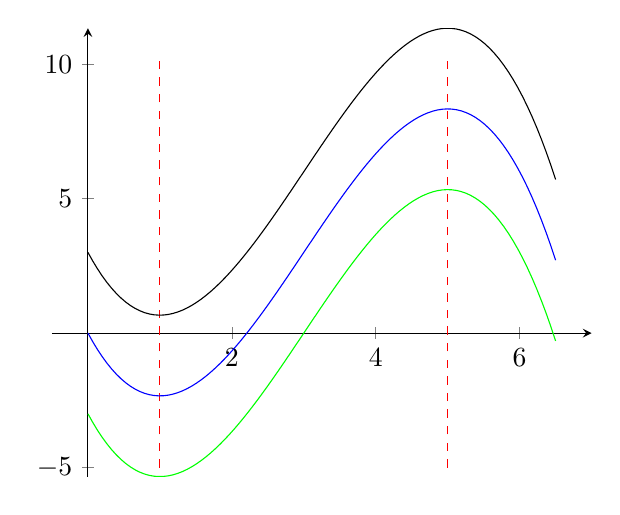
\begin{tikzpicture}
		\begin{axis}[xmin=-0.5, xmax=7, axis lines = center]
		\addplot[red, dashed, samples=50]coordinates{(1,-5) (1, 10.25)};
		\addplot[red, dashed, samples=50]coordinates{(5, -5) (5, 10.25)};
		\addplot[blue, samples=100, domain=0:6.5]{-(1/3)*x^3+3*x^2-5*x};
		\addplot[black, samples=100, domain=0:6.5]{-(1/3)*x^3+3*x^2-5*x+3};
		\addplot[green, samples=100, domain=0:6.5]{-(1/3)*x^3+3*x^2-5*x-3};
		\end{axis}
	\end{tikzpicture}
	\caption{Possible graphs of $f$}
	\label{fig:sketchf5}
\end{figure}

\subsection{Practice Sketching f from f'}
\begin{figure}[htbp]
	\centering
	\begin{tikzpicture}
		\begin{axis}[xmin=-1.2, xmax=8.5, xtick={-1,0,1,2,3,4,5,6,7,8}, xlabel=$x$, 
		ylabel=$f'(x)$, axis lines = center]
		\addplot[blue, samples=100, domain=-0.9:7.9]{(-4/35)*(x-1)*(x-5)*(x-7)*x+4};
		\end{axis}
	\end{tikzpicture}
	\caption{Graph of $f'(x)$}
	\label{fig:sketchex}
\end{figure}


\begin{Exercise}[label=sketch1]
Use figure \ref{fig:sketchex} to answer the following questions:
\begin{enumerate}
\item On what approximate intervals is $f$ increasing or decreasing?
\item At what approximate values of $x$ does $f$ have a local maximum or minimum?
\item Sketch a possible graph of $f$ in the space below:
\end{enumerate}
\end{Exercise}

\begin{tikzpicture}
\begin{axis}[axis lines = left, ylabel=$f(x)$, xlabel=$x$, ticks=none]
\end{axis}
\end{tikzpicture}

\begin{Answer}[ref=sketch1]
[Your answers are meant to be estimates; anything within $\pm 0.1$ of the given 
answers are reasonable estimates.]
\begin{enumerate}
	\item $f(x)$ is increasing on the intervals $x\in (-0.5, 2.2)\cup(4, 7.3)$. 
	$f(x)$ is decreasing on the intervals $x\in (-\infty, -0.5)\cup(2.2, 4)\cup(
	7.3, \infty)$. 
	\item $f(x)$ has local maxima at $x = 2.2, 7.3$ and local minima at $x=-0.5, 
	4$. 
	\item Your sketch should show the maxima and minima identified in part 2. One 
	possible solution is shown below.
	\begin{tikzpicture}
	\begin{axis}[xtick={-1,0,1,2,3,4,5,6,7,8}, ytick={}, xmin=-1.2, xmax=8.5]
	\addplot[blue, samples=100, domain=-0.9:7.9]{-4*(x^5)/175+13*(x^4)/35-188*(x^3
	)/105+2*x^2+3.5*x};
	\end{axis}
	\end{tikzpicture}
\end{enumerate}
\end{Answer}	

\section{Using second derivatives to describe a function}
\subsection{Concavity}
Let's examine two increasing functions, $f(x) = \frac{x^2}{2}$ and $g(x) = 
\sqrt{x}$:
\begin{figure}
\centering
\begin{tikzpicture}
\begin{axis}[xmin=0, xmax=4, ymin=0, ymax=4, axis lines=center]
\addplot[blue, samples=100, domain=0:4]{x^2/2};
\addlegendentry{$f(x)=\frac{x^2}{2}$}
\addplot[red, samples=100, domain=0:4]{sqrt(x)};
\addlegendentry{$g(x)=\sqrt{x}$}
\end{axis}
\end{tikzpicture}
\end{figure}

Even though both of these functions are increasing, they have different shapes. 
$f(x)$ looks like a bowl. On the other hand, $g(x)$ looks like an upside-down 
bowl. These shapes are called \textit{concave up} (in the case of $f(x)$) and 
\textit{concave down} (in the case of $g(x)$). Both functions are increasing on 
the interval $x \in [0, 4]$, and therefore both $f'(x)$ and $g'(x)$ are 
positive on the stated interval. Let's look at their second derivatives, $f''(x
)$ and $g''(x)$:

\begin{figure}
\centering
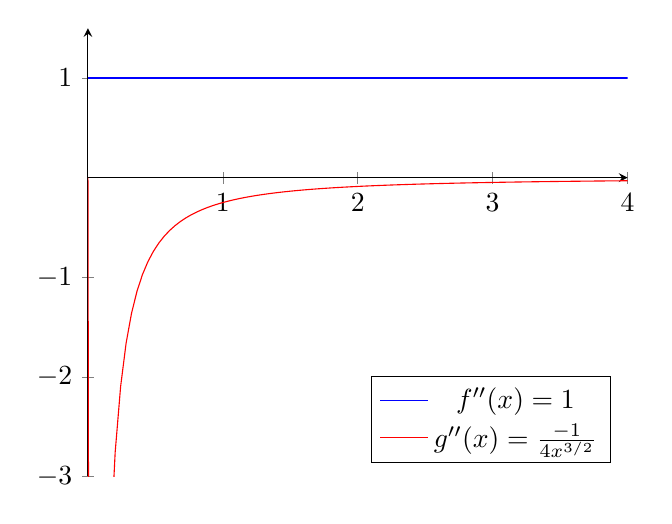
\begin{tikzpicture}
\begin{axis}[xmin=0, xmax=4, ymin=-3, ymax=1.5, axis lines=center, legend pos 
= south east]
\addplot[blue, samples=100, domain=0:4]{1};
\addlegendentry{$f''(x)=1$}
\addplot[red, samples=100, domain=0:4]{(-0.25)*(x^(-3/2)};
\addlegendentry{$g''(x)=\frac{-1}{4x^{3/2}}$}
\end{axis}
\end{tikzpicture}
\end{figure}

As you can see, $f''(x) >0$ and $g''(x)<0$. The second derivative tells us if 
a function is concave up or concave down. In general:
\begin{enumerate}
\item If $f''(x)>0$ for all $x$ in a given interval, then the graph of $f$ is 
concave up on the interval.
\item If $f''(x)<0$ for all $x$ in a given interval, then the graph of $f$ is 
concave down on the interval.
\end{enumerate}

Additionally, the second derivative can help us determine if there is a local 
minimum or maximum at critical numbers. Look at the graphs of $f(x) = 2-x^2$ 
and $g(x) = x^2$, which both have first derivatives equal to $0$ at $x=0$:
\begin{figure}
\centering
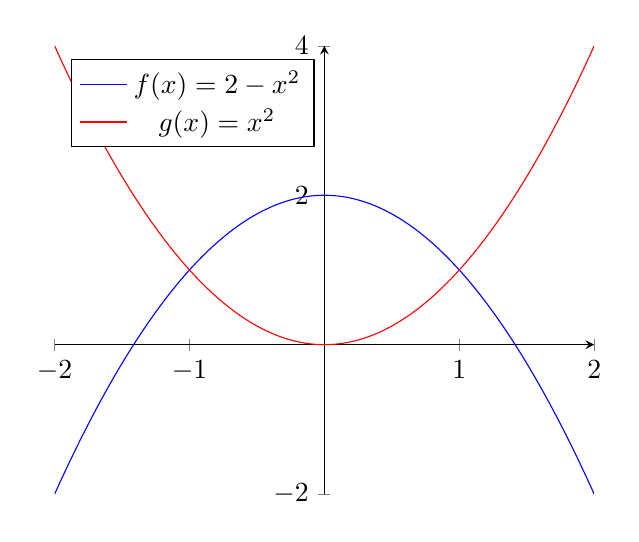
\begin{tikzpicture}
\begin{axis}[xmin=-2, xmax=2, axis lines=center, legend pos = north west]
\addplot[blue, samples=100, domain=-2:2]{2-x^2};
\addlegendentry{$f(x)=2-x^2$}
\addplot[red, samples=100, domain=-2:2]{x^2};
\addlegendentry{$g(x)=x^2$}
\end{axis}
\end{tikzpicture}
\end{figure}

When the graph is concave up, there is a local minimum where the first 
derivative equals $0$. When the graph is concave down, there is a local 
maximum where the first derivative equals $0$. This is summarized with the 
Second Derivative Test:

Suppose $f''$ is continuous near $c$. Then,
\begin{enumerate}
\item If $f'(c) = 0 \text{ and } f''(c)>0$, then $f$ has a local minimum at $c$.
\item If $f'(c) =0 \text{ and } f''(c)<0$, then $f$ has a local maximum at $c$. 
\end{enumerate}


\subsection{Inflection Points}
If $f$ is concave up when $f''>0$ and concave down when $f''<0$, what about 
when $f''=0$? This is the value at which $f$ changes from concave up to concave 
down (or vice versa), which is called an \textit{inflection point}. Similar to 
local extrema with $f'$, if there is an inflection point at $x=c$, then $f''(c)
=0$, but the converse is not necessarily true. To check if $x=c$ is an 
inflection point, then $f''$ should change signs on either side of $x=c$ (
either from positive to negative to from negative to positive). 

Look at the graph of $f(x) = x^4-4x^3$. The concave up areas are shown in red, 
and the concave down in blue:

\begin{figure}[htbp]
\centering
\begin{tikzpicture}
\begin{axis}[axis lines = center, xmin = -2, xmax=5]
\addplot[red, samples=50, domain=-1.5:0]{x^4-4*x^3};
%fixme label inflection points
\addplot[black, mark=*]coordinates{(0,0)};
\addplot[blue, samples=50, domain=0:2]{x^4-4*x^3};
\addplot[black, mark=*]coordinates{(2, -16)};
\addplot[red, samples=50, domain=2:4.25]{x^4-4*x^3};
\end{axis}
\end{tikzpicture}
\end{figure}
Let's examine $f''$ to confirm the inflection points are at $(0, 0)$ and $(2, 
-16)$. First, we note that $f''(x) = 12x^2-24x$. Factoring, we see that $f''(x) 
= 12x(x-2)$, which has zeroes at $x=0$ and $x=2$. For $x<0$, $f''>0$, and for 
$0<x<2$, $f''<0$; therefore, there is an inflection point in $f$ at $(0, 0)$. 

\begin{Exercise}[label=concavity1]
Prove that the other inflection point for $f(x) = x^4-4x^3$ is $(2, -16)$.
\end{Exercise}

\begin{Answer}[ref=concavity1]
Noting that $f''(2)=0$, we examine the value of $f''$ around $x=2$. For $0<x<2$
, $f''<0$, which indicates $f$ is concave down in the domain $x \in (0,2)$. For 
$x>2$, $f''>0$, which indicates $f$ is concave up. Therefore, there is an 
inflection point at $x=2$ for $f$. Recalling that $f(x) = x^4-4x^3$, we find 
the coordinate of the inflection point by substituting $x=2$:
$$f(2) = 2^4-4*2^3=16-4*8=16-32=-16$$
Therefore, $f(x)$ has an inflection point at $(2, -16)$.
\end{Answer}

\begin{Exercise}[label=concavity2]
	The graph below shows $g'(x)$. Describe the behavior of $g(x)$ from $x=0$ 
	to $x=2$. 
	\begin{tikzpicture}
		\begin{axis}[axis lines = center, xmin=0, xmax=2, xlabel=$x$, ylabel=$g'(x)$]
		\addplot[blue, samples=100, domain=0:2]{sqrt(x)};
		\end{axis}
	\end{tikzpicture}
\end{Exercise}

\begin{Answer}[ref=concavity2]
	According to the graph, $g'$ is positive and increasing. Therefore, $g$ is 
	increasing (because $g'$ is positive) and concave up (because $g'$ is 
	increasing, and therefore $g''$ is positive).
\end{Answer}

\begin{Exercise}[label = concavity3]
[This question was originally presented as a calculator-allowed, multiple-choice 
problem on the 2012 AP Calculus BC exam.] For $-1.5 < x < 1.5$, let $f$ be a 
function with first derivative given by $f'(x) = e^{(x^4 - 2x^2 + 1)} - 2$. State 
the interval(s) (to three decimal places) for which $f$ is concave down. 
\end{Exercise}

\begin{Answer}[ref = concavity3]
Since the question asks about concavity, we need to examine the second derivative:
$$f''(x) = \frac{d}{dx} f'(x) = \frac{d}{dx} \left[ e^{(x^4 - 2x^2 + 1)} - 2 
\right]$$
$$f''(x) = \left( x^4 - 2x^2 + 1 \right) e^{(x^4 - 2x^2 + 1)} \left(4x^3 - 4x 
\right)$$

The second derivative equals zero when $x^4 - 2x^2 + 1 = (x^2 - 1)^2 = 0$ or 
$4x^3 - 4x = 4(x)(x^2-1) = 0$, which gives roots $x = 0$, $x = 1$, and $x = 
-1$. So the intervals we need to test are $(-1.5, -1)$, $(-1, 0)$, $(0, 1)$, 
and $(1, 1.5)$. To test $x \in (-1.5, -1)$, we will substitute $x = -1.25$ 
into $f''(x)$:
$$f''(-1.25) = -3.85928 < 0$$
Therefore, $f(x)$ is concave down on the interval $x \in (-1.5, -1)$. 
Next, we test $x \in (-1, 0)$:
$$f''(-0.5) = 2.63258 > 0$$
So, we eliminate $x \in (-1, 0)$. Next, we test $x \in (0, 1)$:
$$f''(0.5) = -2.63258 < 0$$
And $f(x)$ is concave down on the interval $x \in (0, 1)$. Finally, we test 
the interval $x \in (1, 1.5)$:
$$f''(1.25) = 3.85928 > 0$$
Which eliminates that interval. Therefore, $f(x)$ is concave down on the 
intervals $x \in (-1.5, -1)$ and $x \in (0, 1)$. 
\end{Answer}

\begin{Exercise}[label = shape1]
[The following problem was originally presented as a calculator-allowed, 
multiple-choice question on the 2012 AP Calculus BC exam.] Consider the 
function, $f$, whose graph is shown below. Classify each of the following 
statements as true or false and explain. 
\begin{enumerate}
\item $f' > 0$ for $x \in (-2, 0)$.
\item $f$ is differentiable at $x = 0$.
\item $f''$ > 0 for $x \in (0, 2)$
\item $f$ has a critical value at $x = 0$
\end{enumerate}
\begin{tikzpicture}
	\begin{axis}[xmin = -2.25, xmax = 2.25, ymin = -0.5, ymax = 2, axis lines = 
	center, xlabel = $x$, x label style = {anchor = north}, xtick = {-2, -1, 1, 2}, 
	ylabel = $f(x)$, ytick = {1}]
        \addplot[blue, thick, domain = -2:0]{-(0.5*x + 1)^2 + 1.5};
        \addplot[blue, thick, domain = 0:1.999]{-sqrt(4 - x^2) + 2.5};
        \end{axis}
    \end{tikzpicture}
\end{Exercise}

\begin{Answer}[ref = shape1]
\begin{enumerate}
\item False. For $x \in (-2, 0)$, the slope of $f(x)$ is negative, which 
implies that $f'(x) < 0$ for $x \in (-2, 0)$.
\item False. The graph comes to a point at $x = 0$, therefore $\lim_{x \to 
0^+} f'(x) \neq \lim_{x \to 0^-} f'(x)$, which means the limit does not 
exist and $f$ is not differentiable at $x = 0$.
\item True. The graph of $f(x)$ is concave up for $x \in (0, 2)$, which means 
the second derivative is positive. 
\item True. Recall that critical values are where derivatives equal 0 or do 
not exist. Since we have established that $f(x)$ does not exist at $x = 0$, 
then there is a critical value at $x = 0$. 
\end{enumerate}
\end{Answer}

\begin{Exercise}[label = shape2]
[The following problem was originally presented as a calculator-allowed, 
multiple-choice question on the 2012 AP Calculus BC exam.] The graph of $f'$, 
the derivative of $f$, is shown below. Classify each of the following 
statements as true or false and explain your answer. 

\begin{enumerate}
\item $f$ has a relative minimum at $x = -3$.
\item The graph of $f$ has a point of inflection at $x = -2$.
\item The graph of $f$ is concave down for $0 < x < 4$.
\end{enumerate}

\begin{tikzpicture}
	\begin{axis}[xmin = -4.25, xmax = 4.25, ymin = -5, ymax = 5, axis lines = 
	center, xlabel = $x$, x label style = {anchor = north}, xtick = {-4, -3, -2, 
	-1, 1, 2, 3, 4}, xticklabels = { , , , , 1, , , }, ylabel = $f(x)$, ytick = 
	\empty]
        \addplot[blue, thick, domain = -4:-2]{-1*(x + 1.75)^2 + 1.55};
        \draw[blue, thick] (-2, 1.5) parabola (-1, 3);
        \addplot[blue, thick, domain = -1:1.75]{-1*x^2 + 4};
        \draw[blue, thick] (1.75, 0.9375) sin (2.5, -0.9);
        \draw[blue, thick] (2.5, -0.9) -- (3, -0.9);
        \draw[blue, thick] (4, -2) sin (3, -0.9);
        \end{axis}
    \end{tikzpicture}
\end{Exercise}

\begin{Answer}[ref = shape2]
\begin{enumerate}
\item True. $f'(3) = 0$ and $f'$ has a positive slope, which means there is a 
local extreme and $f$ is concave up at $x = 3$. Therefore, there is a local 
minimum at $x = 3$.
\item False. Though it appears that $f'' = 0$ at $x = -2$, the slope of $f'$ 
is positive before and after. Therefore, $f''$ does not cross the $x$-axis 
and there is not an inflection point at $x = -2$. 
\item True. For $ 0 < x < 4$, the slope of $f'$ is negative, which means 
$f''$ is negative, which means $f$ is concave down. 
\end{enumerate}
\end{Answer}

\begin{Exercise}[label = shape3]
[The following problem was originally presented as a calculator-allowed, 
multiple-choice question on the 2012 AP Calculus BC exam.] Let $f$ be a 
function that is twice differentiable on $-2 < x< 2$ and satisfies the 
conditions in the table below. If $f(x) = f(-x)$, what are the $x$-coordinates 
of the points of inflection of the graph of $f$ on $-2 < x < 2$?

\begin{tabular}{|c|c|c|}\hline
 & $0 < x < 1$ & $1 < x < 2$\\\hline
 $f(x)$ & Positive & Negative\\\hline
 $f'(x)$ & Negative & Negative\\\hline
 $f''(x)$ & Negative & Positive\\\hline
\end{tabular}
\end{Exercise}

\begin{Answer}[ref = shape3]
The graph of $f$ has inflection points at $x = -1$ and $x = 1$. Since $f(x) = 
f(-x)$, we can expand the table to include the entire window we are 
investigating:
\begin{tabular}{|c|c|c|c|c|}\hline
 & $-2 < x < -1$ & $-1 < x < 0$ & $0 < x < 1$ & $1 < x < 2$\\\hline
 $f(x)$ & Negative & Positive & Positive & Negative\\\hline
 $f'(x)$ & Negative & Negative & Negative & Negative\\\hline
 $f''(x)$ & Positive & Negative & Negative & Positive\\\hline
\end{tabular}
Recall that inflection points occur when $f''$ changes from positive to 
negative or from negative to positive. Examining the table, we see that the 
sign of $f''$ changes at $x = -1$ and $x = 1$. 
\end{Answer}
